\section{Introduction}
\begin{frame}
  \frametitle{Background and Motivation}

FPGAs are making their way into data centers to boost the computing power
	and the overall power efficiency.

% \begin{itemize}
%       \item Only basic programmability
%       \item Incompatible APIs
%       \item Licensed VHDL code blobs
%       \item Seldom swap-able
%       \item \textbf{Price!}
%     \end{itemize}


\begin{figure}
	\centering
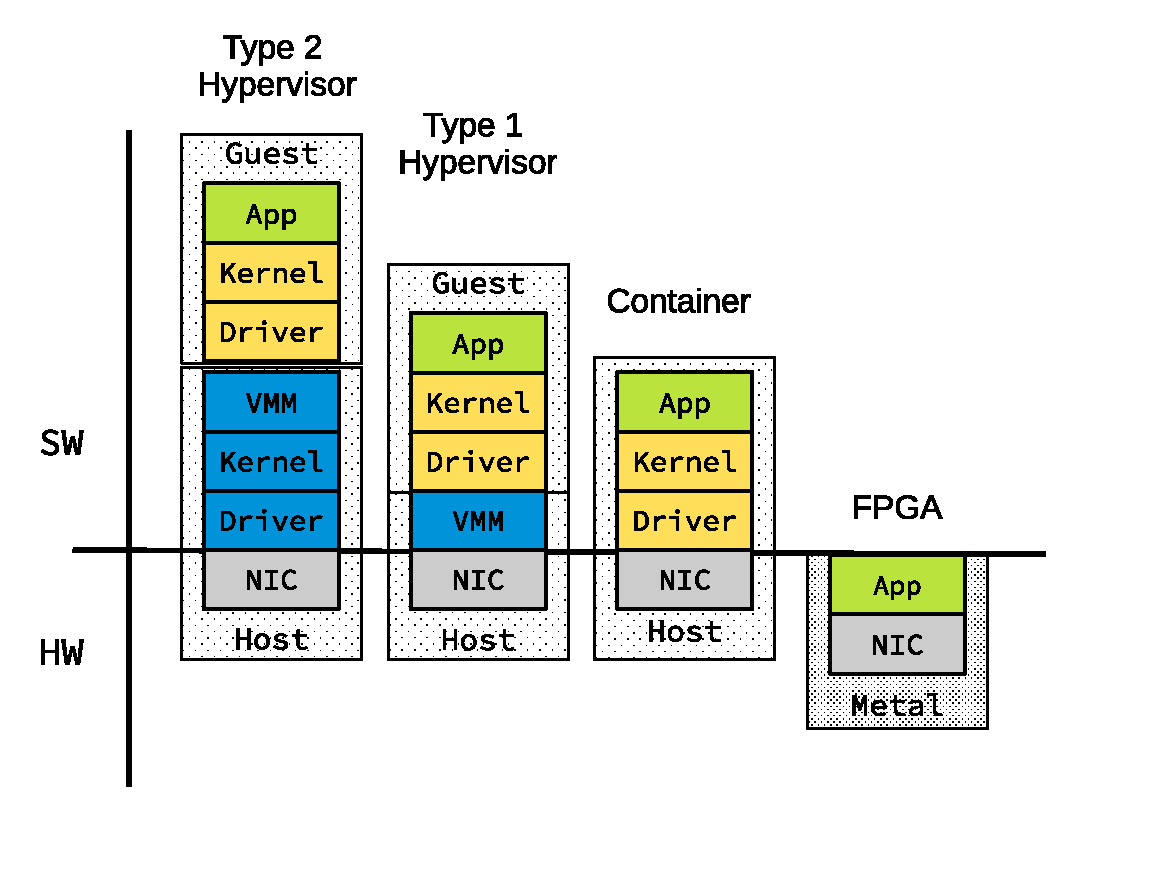
\includegraphics[scale=0.5]{./background/server_configuration.eps}
\end{figure}


\end{frame}


\begin{frame}

A conventional data center architecture
\begin{figure}
	\centering
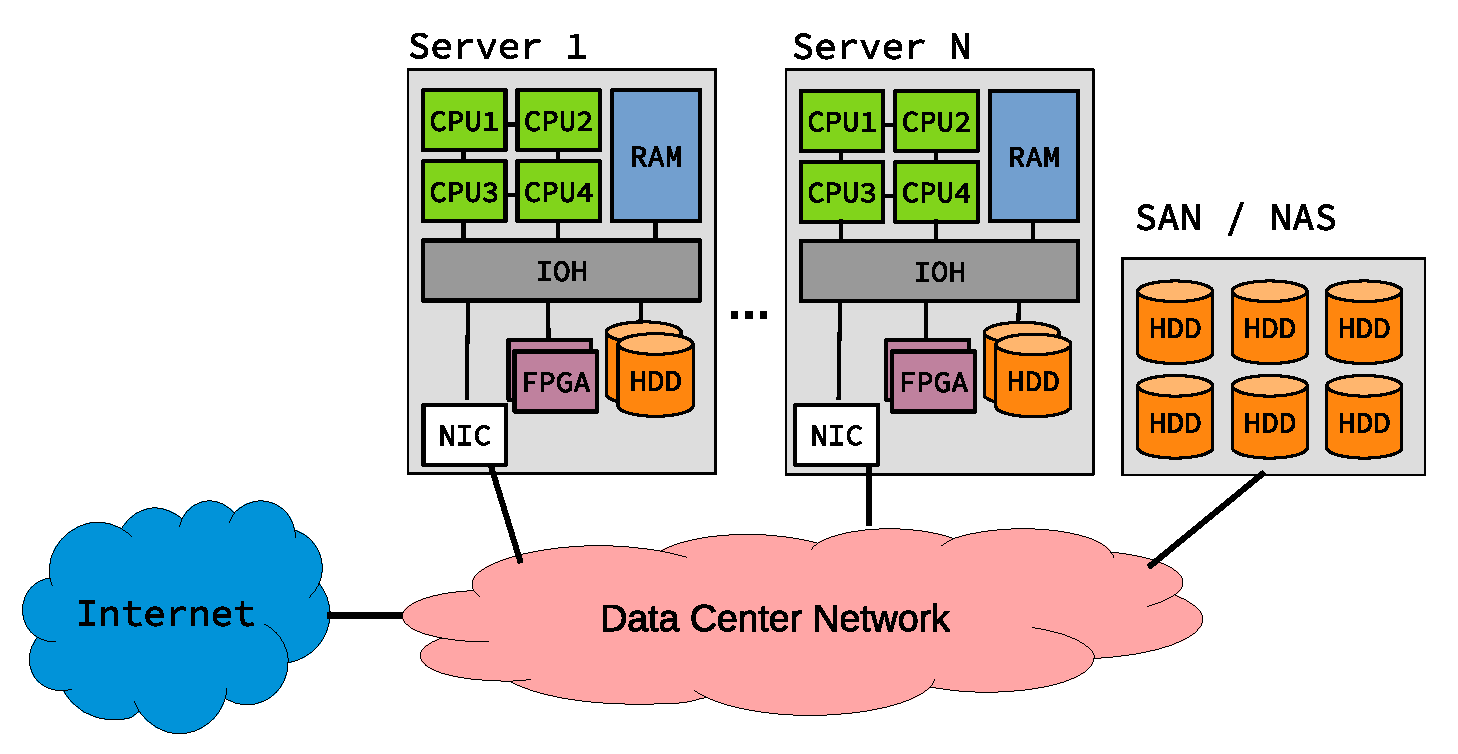
\includegraphics[scale=0.5]{./background/dc_architectures_conventional.eps}
\end{figure}

\end{frame}


\begin{frame}

Proposed, disaggregated data center architecture


\begin{figure}
	\centering
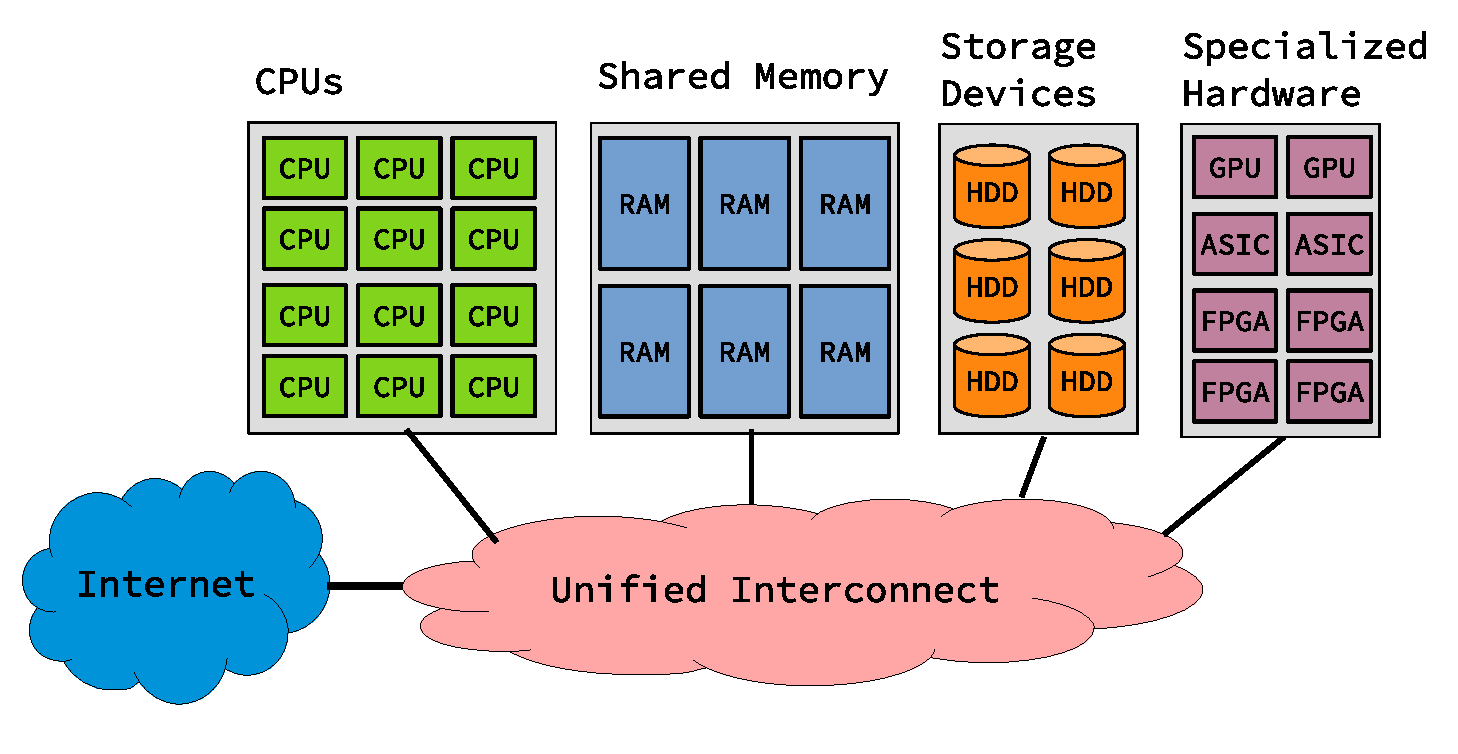
\includegraphics[scale=0.5]{./background/dc_architectures_disaggregated.eps}
\end{figure}



\end{frame}

% - Network Stack Specialization for Performance\\
% - Disaggregated FPGAs\\
% - A Cloud-Scale Acceleration Architecture

% "Intel FPGAs burst open these bottlenecks with a combination of
% microarchitectural flexibility, massive parallelism, huge data bandwidth,
% and rapid reconfigurability. As workloads and traffic pattern shift, Intel
% FPGAs can anticipate needs and bring optimized hardware acceleration to
% bear on the critical points."



% Talking points:
% 1. In the current era of big data, computationally heavy applications are
% moving to the cloud.

% 2. DC infrastructures are being redesigned to pack ever more compute capacity
% into the same volume and power envelops

% 3. This is done by increasing the density of the servers by sharing resources,
% such as power supplies, cooling, fans, networking uplinks, and other management
% infrastructures.

% 4. Problem -- currently, FPGAs are connected directly to CPUs using some PCI
% bus, making the separation hard. [0] proposes FPGA must be turned into a
% self-contained standalone appliance capable of managing itself. Then, it is
% connected to the rest of the Data-Center by a local network.

% 5. In this thesis, we want to make a self-contained TCP/IP stack on an FPGA
% using SME.


% [0]: [Disaggregated FPGAs]


